\documentclass[aspectratio=169]{beamer}
\beamertemplatenavigationsymbolsempty
%\setbeameroption{show only notes}
%\setbeameroption{show notes on second screen}

\usepackage{pdfpages}
\usepackage{graphicx}
\graphicspath{{figures}{figures/graphics}}


\usepackage{tikz}
\usepackage{tikzscale}
\usetikzlibrary{shapes, arrows.meta, positioning, calc, intersections}
\tikzstyle{block} = [rectangle, draw, rounded corners]


\usepackage[export]{adjustbox}

\usepackage{caption}
\captionsetup[figure]{labelformat=empty, font=scriptsize, labelfont=scriptsize}

\usepackage{subcaption}
\usepackage{multicol}

\usepackage[numbers, sort&compress]{natbib}
\bibliographystyle{unsrtabbrv}

\definecolor{palatinatepurple}{rgb}{0.41, 0.16, 0.38}

\hypersetup{
	colorlinks=true,
	linkcolor=black,
	citecolor=black,
	urlcolor=palatinatepurple
}

% beamer style
\setbeamertemplate{blocks}[rounded][shadow]
\setbeamercolor{block body}{bg=structure!10}
\setbeamercolor{block title}{bg=structure!20}

\setbeamercolor{block body example}{bg=green!10}
\setbeamercolor{block title example}{bg=green!20}

\setbeamercolor{block body alerted}{bg=red!10}
\setbeamercolor{block title alerted}{bg=red!20, fg=black}



% just have frame number in footline
\setbeamertemplate{footline}[frame number]

\def\swidth{2cm}
\usetheme[width=\swidth]{Hannover}
%\usecolortheme{}

%%%%% ADD  NOPHOTO Icon

%
\makeatletter
\addtobeamertemplate{sidebar left}{}{%
	\begin{minipage}{\swidth}
		\centering
%		\includegraphics[width=0.3\textwidth]{../../../pres-images/no-photo}
		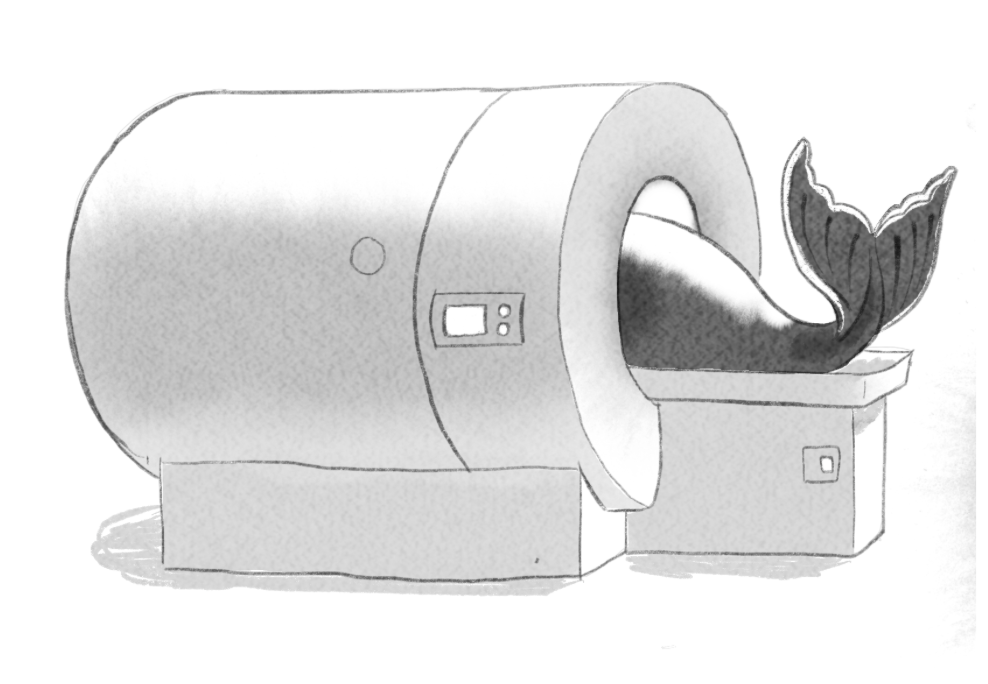
\includegraphics[width=1.5cm]{complexwhale}
		\vspace{2em}
	\end{minipage}
	
}
\makeatother

%%%%%

% numberless footnote
\newcommand\blfootnote[1]{%
	\begingroup
	\renewcommand\thefootnote{}\footnote{#1}%
	\addtocounter{footnote}{-1}%
	\endgroup
}



\title[Brainwise Wordsearch]{Lexical Methodological Exploration of Neuroimaging Studies}
\subtitle[]{PoCS2 Project Proposal}

\date{}

\author[Tony Barrows]{Tony Barrows}

%\institute[UVM]{ 
\includegraphics[width=4cm]{larner}}

%\institute{\inst{1} University of Vermont \and \inst{2} University of Michigan}

\begin{document}
	
	\begin{frame}
		\maketitle
		
		\centering
%		\includegraphics[width=2cm]{../../../pres-images/20150925-ABCD}
		
\includegraphics[width=3cm]{larner}
		
\includegraphics[width=3cm]{nerve}
		
\includegraphics[width=2cm]{complexsystems}
		
\includegraphics[width=2cm]{complexbrain}
%		
\includegraphics[width=2cm]{../../../pres-images/complexsystems}
%		\includegraphics[width=3cm]{../../../pres-images/vacc_green}
	\end{frame}
	
	%% Outline
%\begin{frame}{Outline}
%	\tableofcontents
%\end{frame}

\section{Introduction}

%\begin{frame}{}
%	\tableofcontents
%\end{frame}

\begin{frame}{Motivation}

	Look for neurobiological mechanisms behind individual differences in behavior
	
	\begin{itemize}
		\item Chart normal and abnormal brain and cognitive development
		\item Identify biomarkers for abnormal behavior
		\item Afford opportunities for individualized medicine
	\end{itemize}
	
	\pause
	\begin{block}{}
		Use neuroimaging to help us understand brain-behavior relationships
	\end{block}
\end{frame}

%TODO Add basic neuroimaging study overview

\begin{frame}{(Very) High-level overview of Functional Magnetic Resonance Imaging (fMRI):}
	\includegraphics[width=\linewidth]{mri_diagram}
	\blfootnote{Images from NIMH and \cite{Siden2020}}
\end{frame}

%\begin{frame}{Overview}
%
%	
%	\begin{enumerate}
%		\item Participants complete tasks in the scanner
%		
%		\pause
%		
%		\item We measure changes in very small magnetic fields related to metabolic demand (blood flow after neuronal activity)
%		
%		\pause
%		
%		\item Recording those changes over time creates a time-series for each tiny volume (voxel)
%		
%		\pause
%		
%		\item Use GLMs to relate the task to the brain time-series
%		
%		\pause
%		
%		\item Fit additional models to look for group-level differences
%		
%		\pause
%		
%		\item Draw pictures using these models
%	\end{enumerate}
%	
%	\begin{figure}
%		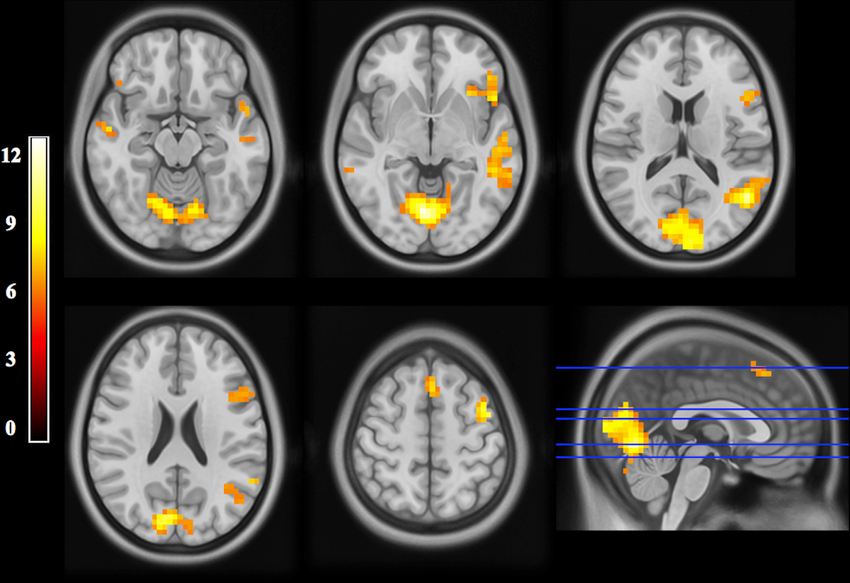
\includegraphics[width=0.3\textwidth]{fmri_ex}
%		\caption{fMRI group-level activation map from \cite{VassalEtAl2016}.}
%	\end{figure}
%	
%\end{frame}


\begin{frame}{Problem}
	\begin{columns}
		\column{0.2\textwidth}
		\includegraphics[width=\columnwidth]{papers/Marek22}
		\column{0.8\textwidth}
		\href{https://www.nature.com/articles/s41586-022-04492-9}{Reproducible brain-wide association studies require thousands of individuals \cite{MarekEtAl2022}}
		
		Reasons:
		\begin{itemize}
			\item Fishing for statistical significance (``p-hacking'') \cite{Nuzzo}
			\item Overfitting \cite{Hawkins2004}
			\item Confirmation and publication biases \cite{Bishop2020}
			\item \textbf<2>{Variability in methods \cite{Botvinik-NezerEtAl2020}} 
		\end{itemize}
	\end{columns}
\end{frame}



% TODO add cartoon of term -> method -> brain





\section{Methods}
%\begin{frame}
%	\tableofcontents
%\end{frame}



\begin{frame}{Automated text-to-brain}

	
	\begin{columns}[t]
		\column{0.5\textwidth}
			
\includegraphics[width=0.5\textwidth]{neurosynth}\cite{YarkoniEtAl2011}
			
			\begin{itemize}
				\item 14,371 studies
				\item 1,334 terms
				\item Focuses on specific inference
			\end{itemize}
			
		\column{0.5\textwidth}
			
\includegraphics[width=0.5\textwidth]{neuroquery}\cite{DockesEtAl2020}
			
			\begin{itemize}
				\item 13,459 studies
				\item 7,547 terms
				\item Focuses on multivariate prediction (across related terms)
				\begin{itemize}
					\item e.g., you enter \texttt{calculation}, it also searches \texttt{computation}
				\end{itemize}
			\end{itemize}
	\end{columns}
	
	\pause
	\begin{block}{}
				Each works by finding relationships between \textbf{terms} and \textbf{brain activation} by extracting standardized coordinates from results
	\end{block}


	\blfootnote{\tiny These numbers may change. It's unclear whether the authors are consistently updating their databases. Many of the same people were involved in each of these efforts.}
\end{frame}

% TODO describe goal

\begin{frame}{Automated text-to...methods?}
	\begin{itemize}
		\item Meta-analysis help overcome problems related to p-hacking, overfitting, and confirmation bias
		\begin{itemize}
			\item $\rightarrow$ but not \textbf{variability in methods}
		\end{itemize}

	\end{itemize}
	
	\vspace{3mm}
	
	\pause
	Proposal:
	
	\begin{itemize}
		\item Use text from \texttt{neurosynth} and \texttt{NeuroQuery} to describe the field:
		\begin{itemize}
			\item Common methods for each type of question
			\item Results patterns associated with different techniques
		\end{itemize}
	\end{itemize}
\end{frame}


\begin{frame}{Things to do}
		
\includegraphics[width=0.15\textwidth]{neuroquery}
		appears to contribute 4,777 \textbf{unique} articles $\ldots$ but with no dates \footnote[1]{%
		\tiny Hours spent writing elegant script to query APIs only to realize the metadata isn't available for a reason: 5+}
		
		\vspace{3mm}
		
		We'll stick with \texttt{neurosynth} for now.
		
		\begin{columns}
			\column{0.75\textwidth}
					\includegraphics[width=\columnwidth]{figures/project/ns_pubcount.pdf}
					
			\column{0.25\textwidth}
				\begin{itemize}
					\item Try to solve $\uparrow$
					\item Generate methods words (buckets)
					\item Drop papers into buckets
					\item Look for developments over time
				\end{itemize}
		\end{columns}

\end{frame}



\begin{frame}[allowframebreaks]{References}

		\tiny
		\bibliography{zotero}

\end{frame}


	
	
\end{document}

